%%%%%%%%%%%%%%%%%%%%%%%%%%%%%%%%%%%%%%%%%%%%%%%%%%%%%%%%%%%%%%%%%%%%%%%%%%%%%%%%%%%%%%%%%
% Section 4: Xilinx Devices
%	This section contains a description of the following:
%	- Vivado FPGA devices (with terminology)
%	- Device data structures in RapidSmith, 
%	- Device files and XDLRC files  
%	- Step-by-step guide on how to intall new devices  
%%%%%%%%%%%%%%%%%%%%%%%%%%%%%%%%%%%%%%%%%%%%%%%%%%%%%%%%%%%%%%%%%%%%%%%%%%%%%%%%%%%%%%%%%
\newpage
\section{Devices}
\graphicspath{{./techReportFigures/sec4_devices/}}

%%%%%%%%%%%%%%%%%%%%%%%%%%%%%%%%%%%%%%%%%%%%%%%%%%%%
% 	Xilinx FPGA Architecture
%%%%%%%%%%%%%%%%%%%%%%%%%%%%%%%%%%%%%%%%%%%%%%%%%%%%
\subsection{Xilinx FPGA Architecture Overview} \label{fpgaArch}
This section is intended to give a brief introduction to Xilinx FPGA
architecture and terminology. The terminology introduced here is consistent
with the terminolgy used in the Vivado Design Suite. If you are already familiar
with Xilinx FPGA devices, then you can skip to \autoref{devicesRS2}. 
As you read through this section, it may be helpful to open a sample device in Vivado's
Device Browser. To do this, open a new command prompt and run Vivado in Tcl mode
(``vivado -mode tcl''). Then, run the following commands in the Vivado prompt:

\begin{lstlisting} [numbers=none,keywordstyle=\ttfamily]
Vivado% link_design -part xc7a100tcsg324-3 -quiet
Vivado% start_gui
\end{lstlisting}

\noindent
Replace ``xc7a100tcsg324-3" with any Xilinx part you are interested in looking
at. After these commands are run, a GUI view should pop up showing the
components of an Artix7 FPGA part. Use this to explore the Xilinx device 
architecture if needed.

% Device Hierarchy
\subsubsection{Device Hierarchy} \label{sec:deviceHierarchy}
Xilinx FPGAs can be broken down into \texttt{series},
\texttt{families}, and individual \texttt{parts}. At the highest level, a series
defines a unique FPGA architecture. Vivado currently supports three different
series: Series7, UltraScale, and UltraScale+. As shown in
\autoref{tab:vivadoFamilies}, each series can be broken down into a list of
families. These families all use the same series architecture, but are
optimized for cost, power, performance, size, or another metric.

\begin{table} [h!]
\caption{Vivado Device Families (organized by series)}
\label{tab:vivadoFamilies}
\vspace{-.15in}
\begin{center}
\begin{tabu}{ |c|c|c|c| }
\hline
\textbf{Series7} & \textbf{UltraScale} & \textbf{UltraScale+} \\
\hline
\hline
 Kintex & Kintex & Kintex \\
 Virtex & Virtex & Virtex \\
 Artix &  &  \\
 Spartan &  &  \\
 Zynq &  &  \\ 
\hline
\end{tabu}
\end{center}
\end{table}

\begin{figure}[b!]
 \centering
 \includegraphics[width=\columnwidth]{deviceHierarchy.png}
 \caption{Xilinx Device Hierarchy}
 \label{fig:deviceHierarchy}
\end{figure}

\noindent Families can further be broken down into one or more parts (actual
FPGA devices). A Xilinx part has a variety of attributes including its number,
package type, and speed-grade. Take the part ``xcku025-ffva1156-1-c'' as an
example. This part is within the Kintex UltraScale family, uses a ``ffva1156''
package type, and has a speed grade of ``1-c''. \autoref{fig:deviceHierarchy}
shows the device hierarchy of a Xilinx part . The following subsections describe
each internal component of a Xilinx FPGA as shown in the figure.

% Tiles
\subsubsection{Tiles}
A Xilinx FPGA is organized into a two-dimensional array of \texttt{Tile}s. Each
tile is a rectangular component of a device that performs a specific function
such as implementing digital logic or storing BRAM memory. Tiles are stamped
across a device  and wired together through the general routing fabric. All
copies of a tile type are identical or nearly identical (they may have minor
routing differences). \autoref{fig:tileExample} displays three types of tiles
in an Artix7 device. The \textbf{VBRK} tile on the left is used for wiring
signals between other tiles (these connections are not programmable). The 
\textbf{INT\_L} tile on the right is a switchbox tile. These are
reconfigurable routing tiles that allow a single wire to be routed to various
locations within the FPGA. The \textbf{CLBLL} tile in the middle is used
to implement combinational and sequential digital logic, and is the fundamental
component of Xilinx FPGAs. Other tile types include DSP, BRAM, FIFO, and IOB.

\begin{figure}[t!]
 \centering
 \includegraphics[width=\columnwidth]{tiles.png}
 \caption{Artix7 Tiles}
 \label{fig:tileExample}
\end{figure}

% Sites
\subsubsection{Sites}
Tiles generally consist of one or more \texttt{Site} objects, which organize
the hardware components of the tile into related groups. Specifically, sites are
the part of a tile which perform the tile's ``useful'' function. The remainder
of the tile is used to wire signals to and from its corresponding sites.
\autoref{fig:site} shows an example site of type SLICEL within a Series7 CLBLL
tile. As the figure shows, a site consists of three main components which are
connected through wires:

\begin{figure}[p!]
\centering
   \begin{subfigure}[h!]{0.85\textwidth}
   \includegraphics[width=\textwidth]{site.png}
   \caption{}
   \label{fig:site1}
\end{subfigure}

\begin{subfigure}[h!]{0.85\textwidth}
   \includegraphics[width=\textwidth]{subsite2.png}
   \caption{}
   \label{fig:site2}
\end{subfigure}

\caption{Series7 SLICEL Site (a), and Highlighted Site Components (b)}
\label{fig:site}
\end{figure}

\begin{itemize}
  \item \textbf{Site} \textbf{PIP}s: Also called routing muxes, these are
  reconfigurable routing PIPs used to specify the internal routing of a site.
  In Vivado, site PIPs are usually configured automatically as cells in a
  design are placed (based on cell properties and placement locations).
  
  \item \textbf{BEL}s: \textbf{B}asic \textbf{EL}ements are hardware components
  within a site for implementing digital logic. For example, look-up-tables
  (LUT) within a SLICEL are used to implement logic equations, and flip-flops
  (FF) are used as storage. In a synthesized netlist, design elements are
  mapped to BELs during implementation.
   
  \item \textbf{Site Pin}s: These pins are connected to wires of the parent tile
  and typically drive/receive signals from the general fabric.
\end{itemize}

\subsubsection{Wires and PIPs} \label{wireSection}
 
\begin{figure}[t!]
	\centering
	\includegraphics[width=0.65\columnwidth]{pipExample.pdf}
	\caption{An example switchbox tile. The green wire represents a source wire,
	and the red wires represent all possible sink wires in the switchbox. The
	highlighed white sections of the figure are PIP connections.}
	\label{fig:switchboxPIP}
\end{figure} 
 
FPGA components are connected together using metal \texttt{Wire}s (called
\texttt{Node}s in Vivado). To make the FPGA reconfigurable,
wires are connected through programmable interconnect points
(PIPs). Individual PIPs can be enabled or disabled as a design is
being routed, and a string of enabled PIPs uniquely identify the
used wires of a physical route. PIPs are most commonly
found in switchbox tiles, and enable a single wire to be
routed to several locations on the chip. \autoref{fig:switchboxPIP}
shows an example switchbox with its corresponding PIPs. The red wires
represent all downhill nodes that the green wire can connect to through a PIP
connection.

%%%%%%%%%%%%%%%%%%%%%%%%%%%%%%%%%%%%%%%%%%%%%%%%%%%%
% 	Device Data Structures
%%%%%%%%%%%%%%%%%%%%%%%%%%%%%%%%%%%%%%%%%%%%%%%%%%%% 
\subsection{Device Data Structures} \label{devicesRS2}
In the original RapidSmith, the device architecture stopped at the
site level. A site was considered a black box who could be
configured using string attributes, but the actual internal components were
unknown. RapidSmith2 extends the device architecture to include all
components \textbf{within} a site as well. \autoref{fig:deviceDataStructures}
shows the new data structure hierarchy, which can be found in the package \emph{
edu.byu.ece.rapidSmith.device}. The classes and interfaces within
\emph{edu.byu.ece.rapid\-Smith.device} are named to reflect the terminology
used by Xilinx. Many classes that exist in Vivado's Tcl interface have a direct map
to a class in RapidSmith2 (such as a \texttt{Tile}). Because of this, most
RapidSmith2 data structures represent a straightforward part of a Xilinx FPGA.
The \texttt{DeviceBrowser} and \texttt{DeviceAnalyzer} example programs
illustrate how to load and browse a device with \texttt{Tile} and \texttt{Site}
data structures, and \autoref{lst:deviceCalls} shows basic device usage in
RapidSmith2. The remainder of this section details important aspects of
RapidSmith2 devices.

% TODO: update this figure to include package pins
\begin{figure}[t]
	\centering
	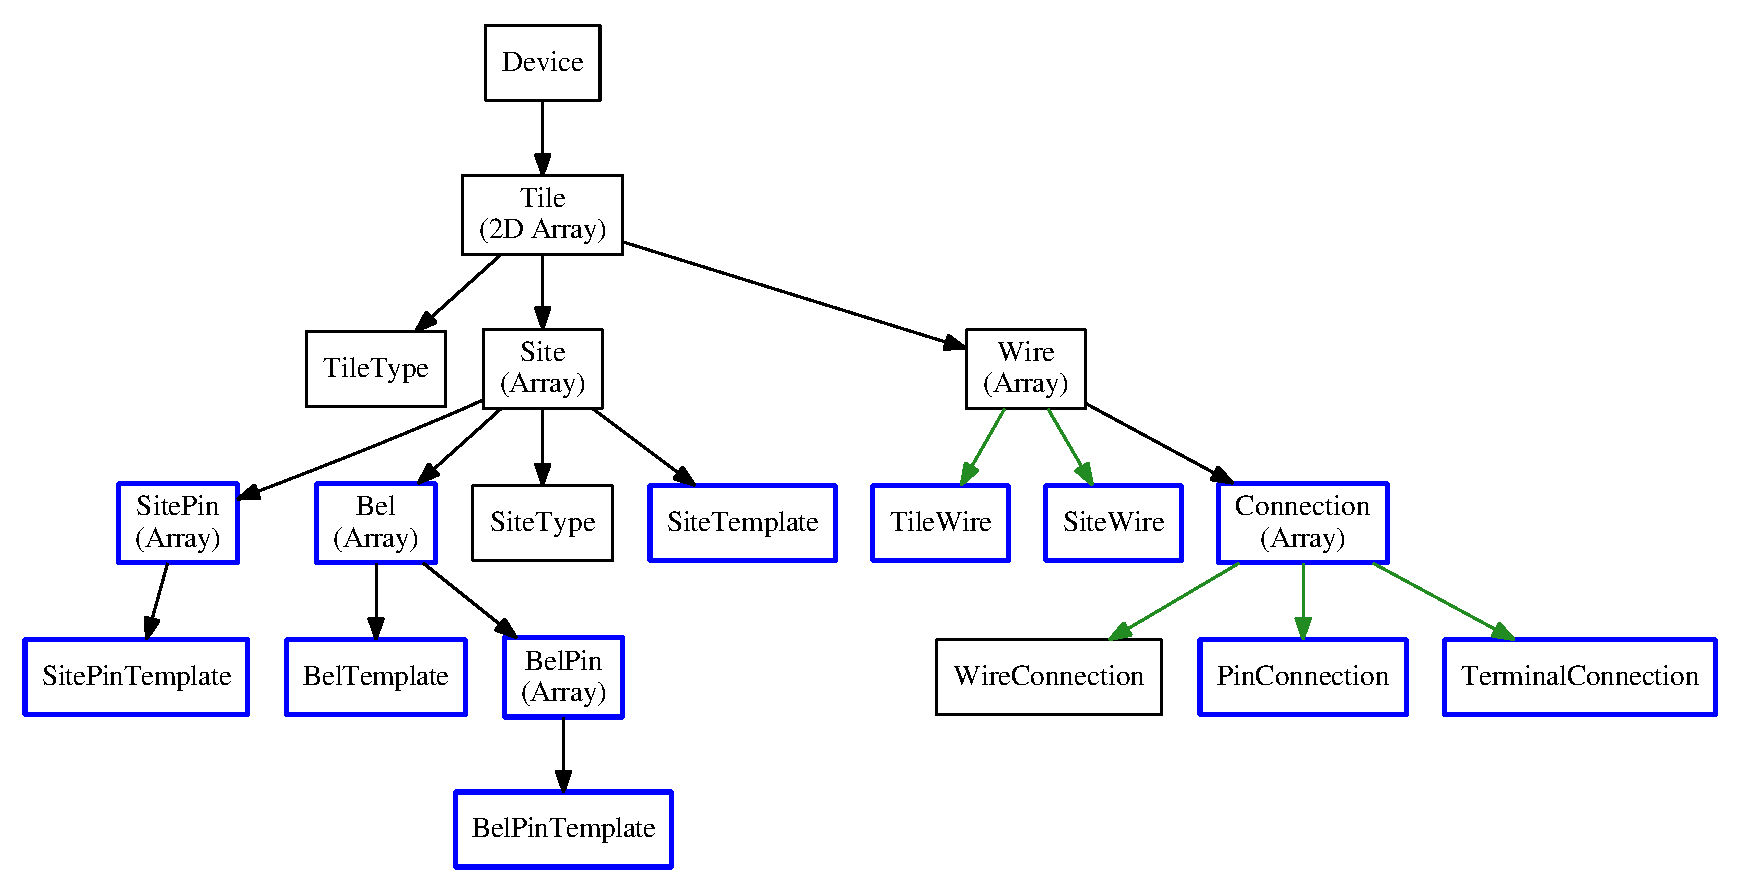
\includegraphics[width=1\columnwidth]{deviceDS.eps}
	\caption{RapidSmith2 Device data structure tree. Green arrows
	represent inheritance, and black arrows represent association. Classes and Interfaces
	bolded in blue are new to RapidSmith 2.}
	\label{fig:deviceDataStructures}
\end{figure}

\begin{lstlisting}[xleftmargin=1.5em, framexleftmargin=1.5em, caption=Basic
device function calls, label=lst:deviceCalls]
  // Get a handle to a device 
  Device device = Device.getInstance("xc7a100tcsg324-3");
	
  // Get device components by name
  Tile tile = device.getTile("CLBLL_R_X27Y130");
  Site site = tile.getSite("SLICE_X44Y130");
  Bel bel = site.getBel("D6LUT");
	
  // Get all device components
  device.getTiles();
  tile.getSites();
  site.getBels();
\end{lstlisting}

\subsubsection{Templates}
As \autoref{fig:deviceDataStructures} shows, there are several template
classes in RapidSmith2. Template classes are used to specify the configuration
of a device structure only once, where the configuration can be reused
across identical objects. The usefulness of templates is best shown with an
example. In an Artix-7 \emph{xc7a100tcsg324} part, there are 11,100 sites of
type SLICEL. Each of these SLICELs have 215 internal components (BELs, pins,
and PIPs). To save memory, RapidSmith2 lazily creates site objects
based on the template only when a handle to a SLICEL site is requested. The
alternative would be to create each of the objects when a device is loaded, but
this would require more memory. Template classes should generally not be
used by the regular user. When creating algorithms using RapidSmith's API, use
the non-template version of classes instead.

\subsubsection{WireEnumerator} \label{wireEnum}
Wires with the same name and function can occur several times throughout a
Xilinx FPGA. For example, the wire \texttt{CLBLL\-\_L\_C2} exists in every tile
of type \texttt{CLBLL\_L} in a Series7 device. To make RapidSmith2
device files small, each uniquely named wire is assigned an integer enumeration
and stored in a \texttt{WireEnumerator} class. The \texttt{WireEnum\-erator}
has methods to convert an integer to the corresponding string wire name and
vice versa.

In previous versions of RapidSmith, the \texttt{WireEnumerator} was used
extensively while building CAD tools. RapidSmith2 has changed this, largely
abstracting the \texttt{WireEnumerator} away in favor of more convenient
methods that return \texttt{Wire} objects which contain a wire's integer
enumeration and name. For example, the name or enumeration of a wire can now be
obtained with the function calls in the \texttt{Wire} interface
\texttt{getWireName()} and \texttt{getWireEnum()} respectively. A handle to the
\texttt{WireEnumerator} still exists in the \texttt{Device} class for those who
want to use it, but this is not recommended.

% TODO: add a code segment here showing the old way vs. new way?

\subsubsection{TileWire and SiteWire} \label{wires}
Wires in RapidSmith2 are uniquely identified not only by their name
(or enumeration), but also by the tile or site in which they exist.
RapidSmith2 introduces the \texttt{TileWire} and \texttt{SiteWire} classes to
encapsulate this information for the user. Many functions in RapidSmith2 now
return a \texttt{TileWire} or \texttt{SiteWire} object (wrapped in a generic
\texttt{Wire}) instead of an integer wire enumeration. \texttt{Wire}s are
connected through \texttt{Connection} objects as described in
\autoref{sec:routing}.

\subsubsection{Package Pins}

Vivado maps all \textit{bonded} IOB sites to corresponding package pins.
Top-level ports of a design can be mapped to these package pins to communicate
with external components. A RapidSmith2 \texttt{Device} object represents Vivado
package pins with \texttt{PackagePin} objects. Each \texttt{PackagePin} 
contains (1) the name of the package pin (i.e. M17), (2) the PAD BEL of the
package pin, and (3) a boolean flag to mark clock package pins. Clock
package pins are those that can access the global clock routing structure of
the FPGA for low skew signals. \autoref{lst:packagePins} shows some available
package pin method calls.

\begin{lstlisting}[xleftmargin=1.5em, framexleftmargin=1.5em,caption=RapidSmith2
package pin functions, label=lst:packagePins] 
  // Get a list of all package pins 
  device.getPackagePins();
	
  // Get a list of clock package pins
  device.getClockPads();
	
  // Get an individual package pin based on the BEL
  Bel bel = device.getSite("IOB_X0Y10").getBel("PAD");
  PackagePin pin = device.getPackagePin(bel);
	
  // Package pin functions
  pin.getName();
  pin.getSite();
  pin.getBel();
  pin.isClockPad();	
\end{lstlisting}

%%%%%%%%%%%%%%%%%%%%%%%%%%%%%%%%%%%%%%%%%%%%%%%%%%%%
% 	Loading a Device
%%%%%%%%%%%%%%%%%%%%%%%%%%%%%%%%%%%%%%%%%%%%%%%%%%%%
\subsection{Loading a Device} \label{sec:loadingDevice}
\autoref{code:loadDevice} below demonstrates how to load a supported device
into RapidSmith2.  The first function call will only load the device into memory
if it has not yet been loaded. If it has been loaded, then the cached
\texttt{Device} data structure will be returned. The second function call will
reload the device from disk, creating a separate \texttt{Device} data
structure. 

\begin{lstlisting}[xleftmargin=1.5em, framexleftmargin=1.5em, caption=Loading a
Device, label=code:loadDevice] 
Device device = RSEnvironment.defaultEnv().getDevice("xc7a100tcsg324");
//or
Device reload = RSEnvironment.defaultEnv().getDevice("xc7a100tcsg324", true);
\end{lstlisting}

\noindent This is useful when implementing multi-threaded code that targets
the same part. \textbf{NOTE:} When a Vivado design is loaded into RapidSmith2
via a RSCP, the corresponding device is also loaded.


%%%%%%%%%%%%%%%%%%%%%%%%%%%%%%%%%%%%%%%%%%%%%%%%%%%%
% 	Supported Device Files
%%%%%%%%%%%%%%%%%%%%%%%%%%%%%%%%%%%%%%%%%%%%%%%%%%%%
\subsection{Supported Device Files} \label{sec:supportedDevices}
RapidSmith2 includes two device files on installation: (1) an Artix7
\texttt{xc7a100tcsg324}, and (2) a Kintex UltraScale \texttt{xcku025-ffva1156}.
These device files have been well tested and are a good starting point for new
users looking to implement Vivado CAD algorithms. However, RapidSmith2 has
general support for the following families:

\begin{multicols}{2}
	\begin{itemize}
	  \item Artix7
	  \item Virtex7
	  \item Kintex7
	  \item Zynq
	  \item Kintex UltraScale
	  \item Virtex UltraScale
 	\end{itemize}
\end{multicols}

\noindent Section \ref{sec:installingNewDevices} describes how to create new
device files for these families and add them to RapidSmith2.